\documentclass{article}
\usepackage{graphicx}
\usepackage{amsmath}
\usepackage{hyperref}
\usepackage{cite}

\graphicspath{{project/paper_images/}}

\title{Deep Learning Project}
\author{
    Group Members: \\
    Farooq Mahmud
}
\date{September 20, 2024}

\begin{document}

\maketitle

\section{Introduction}
Convolutional Neural Networks (CNNs) have become a cornerstone in the field of computer vision, enabling significant advancements in tasks such as image classification. One of the most impactful architectures is the **Inception Network** introduced in the paper ``Going Deeper with Convolutions" by Szegedy et al.~\cite{szegedy2015going}. This architecture, commonly referred to as **GoogLeNet**, achieved remarkable performance in the 2014 ImageNet competition by introducing the concept of multi-scale processing through Inception modules.

The objective of this project is to analyze and replicate the Inception v1 (GoogLeNet) model using TensorFlow, train it on a subset of the ImageNet dataset, and evaluate its performance. Additionally, we will adapt the model to other datasets, such as CIFAR-10, to test its generalization capabilities.


\section{Background}

GoogLeNet introduced a novel approach to convolutional neural networks by stacking multiple Inception modules. Each Inception module consists of parallel branches that apply different-sized convolutional filters (1x1, 3x3, 5x5) and max-pooling operations in parallel. These branches are concatenated to capture multi-scale features.

The Inception module aims to mitigate computational costs by including 1x1 convolutions for dimensionality reduction before performing the larger convolution operations. This was one of the key innovations that made GoogLeNet both efficient and powerful, despite being deeper than previous CNN architectures such as AlexNet and VGGNet~\cite{krizhevsky2012imagenet, simonyan2015vgg}.

\section{Methodology}

\subsection{Image Selection}
The Imagenet dataset contains over 1 million images with a size of over 1TB. Processing this amount of data would not be practical given the available coumputing power. In order to make processing possible in a reasonable timeframe, a subset of the Imagenet images was downloaded. The subsets, or \textit{synsets} map to the CIFAR-10 image classes as shown in Table \ref{tab:synsets}.

\begin{table}[ht]
    \centering
    \begin{tabular}{ll}
    \hline
    \textbf{Synset ID} & \textbf{Equivalent CIFAR-10 Class} \\ \hline
    n02691156 & airplane \\ \hline
    n02958343 & automobile \\ \hline
    n01503061 & bird \\ \hline
    n02121808 & cat \\ \hline
    n02419796 & deer \\ \hline
    n02084071 & dog \\ \hline
    n01641577 & frog \\ \hline
    n02374451 & horse \\ \hline
    n04194289 & ship \\ \hline
    n04467665 & truck \\ \hline
    \end{tabular}
    \caption{Imagenet synset to CIFAR-10 class mapping}
    \label{tab:synsets}
\end{table}

The resulting download consists of 14,738 files with a total size of 1.3GB. Scaling the images to 224 x 224 pixels, the dimensions used by Szegedy, et. al. decreased the size to a manageable 137MB.

After scaling, the images were organized into training, testing, and validation sets. The percentages were 70\% for training, 20\% for testing, and 10\% for validation.

\subsection{A Simple Sequential Network as a Control}
Before constructing a complex model like GoogLeNet, it is a good idea to use a simple network as a baseline. This network is shown in Figure \ref{fig:cnn-control}

\begin{figure}[ht]
    \centering
    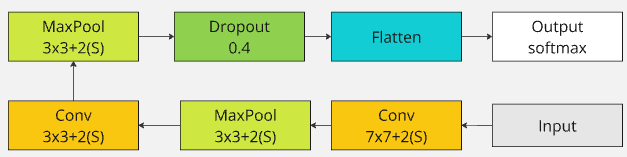
\includegraphics[scale=0.7]{project/paper_images/control_cnn.png}
    \caption{Simple CNN used as a control}
    \label{fig:cnn-control}
\end{figure}

This simple model, when trained wfor 25 epochs, achieved a maximum accuracy of 59\% as shown in Figure \ref{fig:cnn-control-accuracy}.


\begin{figure}[ht]
    \centering
    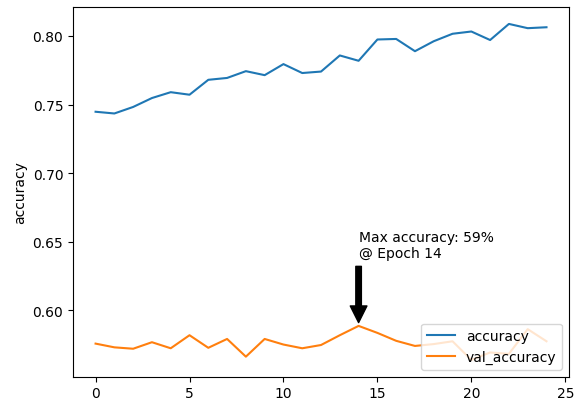
\includegraphics[scale=0.7]{project/paper_images/control_cnn_accuracy.png}
    \caption{Control CNN accuracy}
    \label{fig:cnn-control-accuracy}
\end{figure}


\clearpage



\subsection{Replicating the Inception v1 (GoogLeNet) Model}
The Inception v1 model incorporates branching and parallel operations. As a result, Tensorflow's Sequential  model is inappropriate. Tensorflow's functional API must be used instead.



\bibliographystyle{plain}
\bibliography{project/refs}

\end{document}
